\documentclass[journal,12pt,twocolumn]{IEEEtran}

\usepackage{setspace}
\usepackage{gensymb}
\singlespacing
\usepackage[cmex10]{amsmath}

\usepackage{amsthm}

\usepackage{mathrsfs}
\usepackage{txfonts}
\usepackage{stfloats}
\usepackage{bm}
\usepackage{cite}
\usepackage{cases}
\usepackage{subfig}

\usepackage{longtable}
\usepackage{multirow}

\usepackage{enumitem}
\usepackage{mathtools}
\usepackage{steinmetz}
\usepackage{tikz}
\usepackage{circuitikz}
\usepackage{verbatim}
\usepackage{tfrupee}
\usepackage[breaklinks=true]{hyperref}
\usepackage{graphicx}
\usepackage{tkz-euclide}

\usetikzlibrary{calc,math}
\usepackage{listings}
    \usepackage{color}                                            %%
    \usepackage{array}                                            %%
    \usepackage{longtable}                                        %%
    \usepackage{calc}                                             %%
    \usepackage{multirow}                                         %%
    \usepackage{hhline}                                           %%
    \usepackage{ifthen}                                           %%
    \usepackage{lscape}     
\usepackage{multicol}
\usepackage{chngcntr}
\usepackage{textcomp}
\DeclareMathOperator*{\Res}{Res}

\renewcommand\thesection{\arabic{section}}
\renewcommand\thesubsection{\thesection.\arabic{subsection}}
\renewcommand\thesubsubsection{\thesubsection.\arabic{subsubsection}}

\renewcommand\thesectiondis{\arabic{section}}
\renewcommand\thesubsectiondis{\thesectiondis.\arabic{subsection}}
\renewcommand\thesubsubsectiondis{\thesubsectiondis.\arabic{subsubsection}}


\hyphenation{op-tical net-works semi-conduc-tor}
\def\inputGnumericTable{}                                 %%

\lstset{
%language=C,
frame=single, 
breaklines=true,
columns=fullflexible
}
\begin{document}

\newcommand{\BEQA}{\begin{eqnarray}}
        \newcommand{\EEQA}{\end{eqnarray}}
\newcommand{\define}{\stackrel{\triangle}{=}}
\bibliographystyle{IEEEtran}
\raggedbottom
\setlength{\parindent}{0pt}
\providecommand{\mbf}{\mathbf}
\providecommand{\pr}[1]{\ensuremath{\Pr\left(#1\right)}}
\providecommand{\qfunc}[1]{\ensuremath{Q\left(#1\right)}}
\providecommand{\sbrak}[1]{\ensuremath{{}\left[#1\right]}}
\providecommand{\lsbrak}[1]{\ensuremath{{}\left[#1\right.}}
\providecommand{\rsbrak}[1]{\ensuremath{{}\left.#1\right]}}
\providecommand{\brak}[1]{\ensuremath{\left(#1\right)}}
\providecommand{\lbrak}[1]{\ensuremath{\left(#1\right.}}
\providecommand{\rbrak}[1]{\ensuremath{\left.#1\right)}}
\providecommand{\cbrak}[1]{\ensuremath{\left\{#1\right\}}}
\providecommand{\lcbrak}[1]{\ensuremath{\left\{#1\right.}}
\providecommand{\rcbrak}[1]{\ensuremath{\left.#1\right\}}}
\theoremstyle{remark}
\newtheorem{rem}{Remark}
\newcommand{\sgn}{\mathop{\mathrm{sgn}}}
\providecommand{\abs}[1]{\vert#1\vert}
\providecommand{\res}[1]{\Res\displaylimits_{#1}}
\providecommand{\norm}[1]{\lVert#1\rVert}
%\providecommand{\norm}[1]{\lVert#1\rVert}
\providecommand{\mtx}[1]{\mathbf{#1}}
\providecommand{\mean}[1]{E[#1]}
\providecommand{\fourier}{\overset{\mathcal{F}}{ \rightleftharpoons}}
%\providecommand{\hilbert}{\overset{\mathcal{H}}{ \rightleftharpoons}}
\providecommand{\system}{\overset{\mathcal{H}}{ \longleftrightarrow}}
%\newcommand{\solution}[2]{\textbf{Solution:}{#1}}
\newcommand{\solution}{\noindent \textbf{Solution: }}
\newcommand{\cosec}{\,\text{cosec}\,}
\providecommand{\dec}[2]{\ensuremath{\overset{#1}{\underset{#2}{\gtrless}}}}
\newcommand{\myvec}[1]{\ensuremath{\begin{pmatrix}#1\end{pmatrix}}}
\newcommand{\mydet}[1]{\ensuremath{\begin{vmatrix}#1\end{vmatrix}}}
\numberwithin{equation}{subsection}
\makeatletter
\@addtoreset{figure}{problem}
\makeatother
\let\StandardTheFigure\thefigure
\let\vec\mathbf
\renewcommand{\thefigure}{\theproblem}
\def\putbox#1#2#3{\makebox[0in][l]{\makebox[#1][l]{}\raisebox{\baselineskip}[0in][0in]{\raisebox{#2}[0in][0in]{#3}}}}
\def\rightbox#1{\makebox[0in][r]{#1}}
\def\centbox#1{\makebox[0in]{#1}}
\def\topbox#1{\raisebox{-\baselineskip}[0in][0in]{#1}}
\def\midbox#1{\raisebox{-0.5\baselineskip}[0in][0in]{#1}}
\vspace{3cm}
\title{AI1103 Assignment-3}
\author{SRIVATSAN T - CS20BTECH11062}
\maketitle
\newpage
\bigskip
\renewcommand{\thefigure}{\theenumi}
\renewcommand{\thetable}{\theenumi}
Download all python codes from
\begin{lstlisting}
https://github.com/CS20BTECH11062/AI1103/tree/main/Assignment-3/codes
\end{lstlisting}
%
and latex-tikz codes from
%
\begin{lstlisting}
https://github.com/CS20BTECH11062/AI1103/tree/main/Assignment-3/Assignment-3.tex
\end{lstlisting}
\section*{QUESTION (GATE-MA-2014-36)}
The time to failure, in months, of lights bulbs \\manufactured at two plants A and B
obey the exponential distributions with means 6 and 2 months respectively. Plant B produces
four times as many bulbs as plant A does. Bulbs from these two plants are indistinguishable.
They are mixed and sold together. Given that a bulb purchased at random is working after 12 months, What is the probability that it was manufactured in plant A?
\section*{SOLUTION}
This problem involves Bayes theorem and \newline Exponential distribution
\bigskip
\begin{itemize}
    \item Probability that bulb is from Plant A =\newline $\pr{A}$ = \(\frac{1}{5}\)
    \item Probability that bulb is from Plant B =\newline$\pr{B}$ = \( \frac{4}{5} \)
\end{itemize}
\bigskip
One can use exponential distribution to find out the probability that the bulbs work after 12 months\\
Let X be a variable representing the lifetime of a bulb in months.\\
So X has a Cumulative distribution Function:
\begin{equation}
    F(x,\lambda) =
    \begin{cases}
        1 - {e}^{-\displaystyle\lambda x} & if \hspace{0.3cm}x \geq 0\\
        0       & if \hspace{0.3cm}x < 0
    \end{cases}
\end{equation}
Where
\begin{itemize}
    \item $\frac{1}{\displaystyle\lambda}$ = Mean of distribution
    \newline
    \item x = Time to failure (in months)
\end{itemize}
\bigskip
So,
\begin{align}
    \lambda_A = \frac{1}{6} , \lambda_B = \frac{1}{2}
\end{align}
\begin{align}
    \pr{X\leq k} = F(X,\lambda)
\end{align}
\begin{center}
    Pr(Works after 12 months $\mid$ A) = \newline 1 - Pr(Fails within 12 months $\mid$ A)\\
\end{center}
\begin{align}
    =& 1 - F(12,\lambda_A)\\
    =& {e}^{\displaystyle - \lambda_A \times 12}\\
    =& {e}^{-2}
\end{align}
\begin{center}
    Pr(Works after 12 months $\mid$ B) = \newline 1 - Pr(Fails within 12 months $\mid$ B)
\end{center}
\begin{align}
    =& 1 - F(12,\lambda_B)\\
    =& {e}^{\displaystyle -\lambda_B \times 12}\\
    =& {e}^{-6}
\end{align}
Lets denote the bulb works after 12 months with the variable W. From Bayes theorem,\\
\begin{align}
    Pr(A \mid W) = & \displaystyle{\frac{Pr(A) \times Pr(W \mid A)}{Pr(A) \times Pr(W \mid A) + Pr(B) \times Pr(W \mid B)}}\\
    = & \displaystyle{\frac{ \displaystyle{\frac{1}{5}} \times {e}^{-2}}{\displaystyle{\frac{1}{5}} \times {e}^{-2} + \displaystyle{\frac{4}{5}} \times {e}^{-6}}}\\[0.5cm]
    = & 0.932
\end{align}
So the probability that the Bulb is manufactured in Plant A given that it works after a year is 0.932.
\pagebreak
%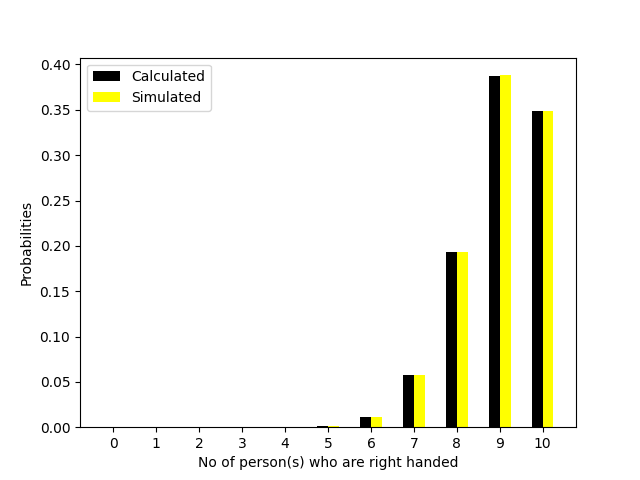
\includegraphics{Figure-1.png}
\end{document}